\documentclass[12pt,UTF8]{ctexart}
\usepackage{ctex,amsmath,amssymb,geometry,fancyhdr,bm,amsfonts
,mathtools,extarrows,graphicx,url,enumerate,color,float,multicol,rotating,subfig} 
\allowdisplaybreaks[4]
% 加入中文支持
\newcommand\Set[2]{\{#1\ \vert\ #2 \}}
\newcommand\Lim[0]{\lim\limits_{n\rightarrow\infty}}
\newcommand\LIM[2]{\lim\limits_{#1\rightarrow#2}}
\newcommand\Ser[1]{\sum_{n=#1}^\infty}
\newcommand{\SER}[2]{\sum_{#1=#2}^\infty}
\newcommand{\Int}[4]{\int_{#1}^{#2}#3\mathrm d#4}
\newcommand{\md}[0]{\mathrm d}
\geometry{a4paper,scale=0.80}
\pagestyle{fancy}
\rhead{多元函数微分学(3)}
\lhead{基础习题课期末复习}
\chead{微积分B(2)}
\begin{document}
\setcounter{section}{2}
\section{方向导数、梯度、映射的微分、泰勒公式}
\noindent
\subsection{复习计划}
\begin{figure}[H]
\begin{center}
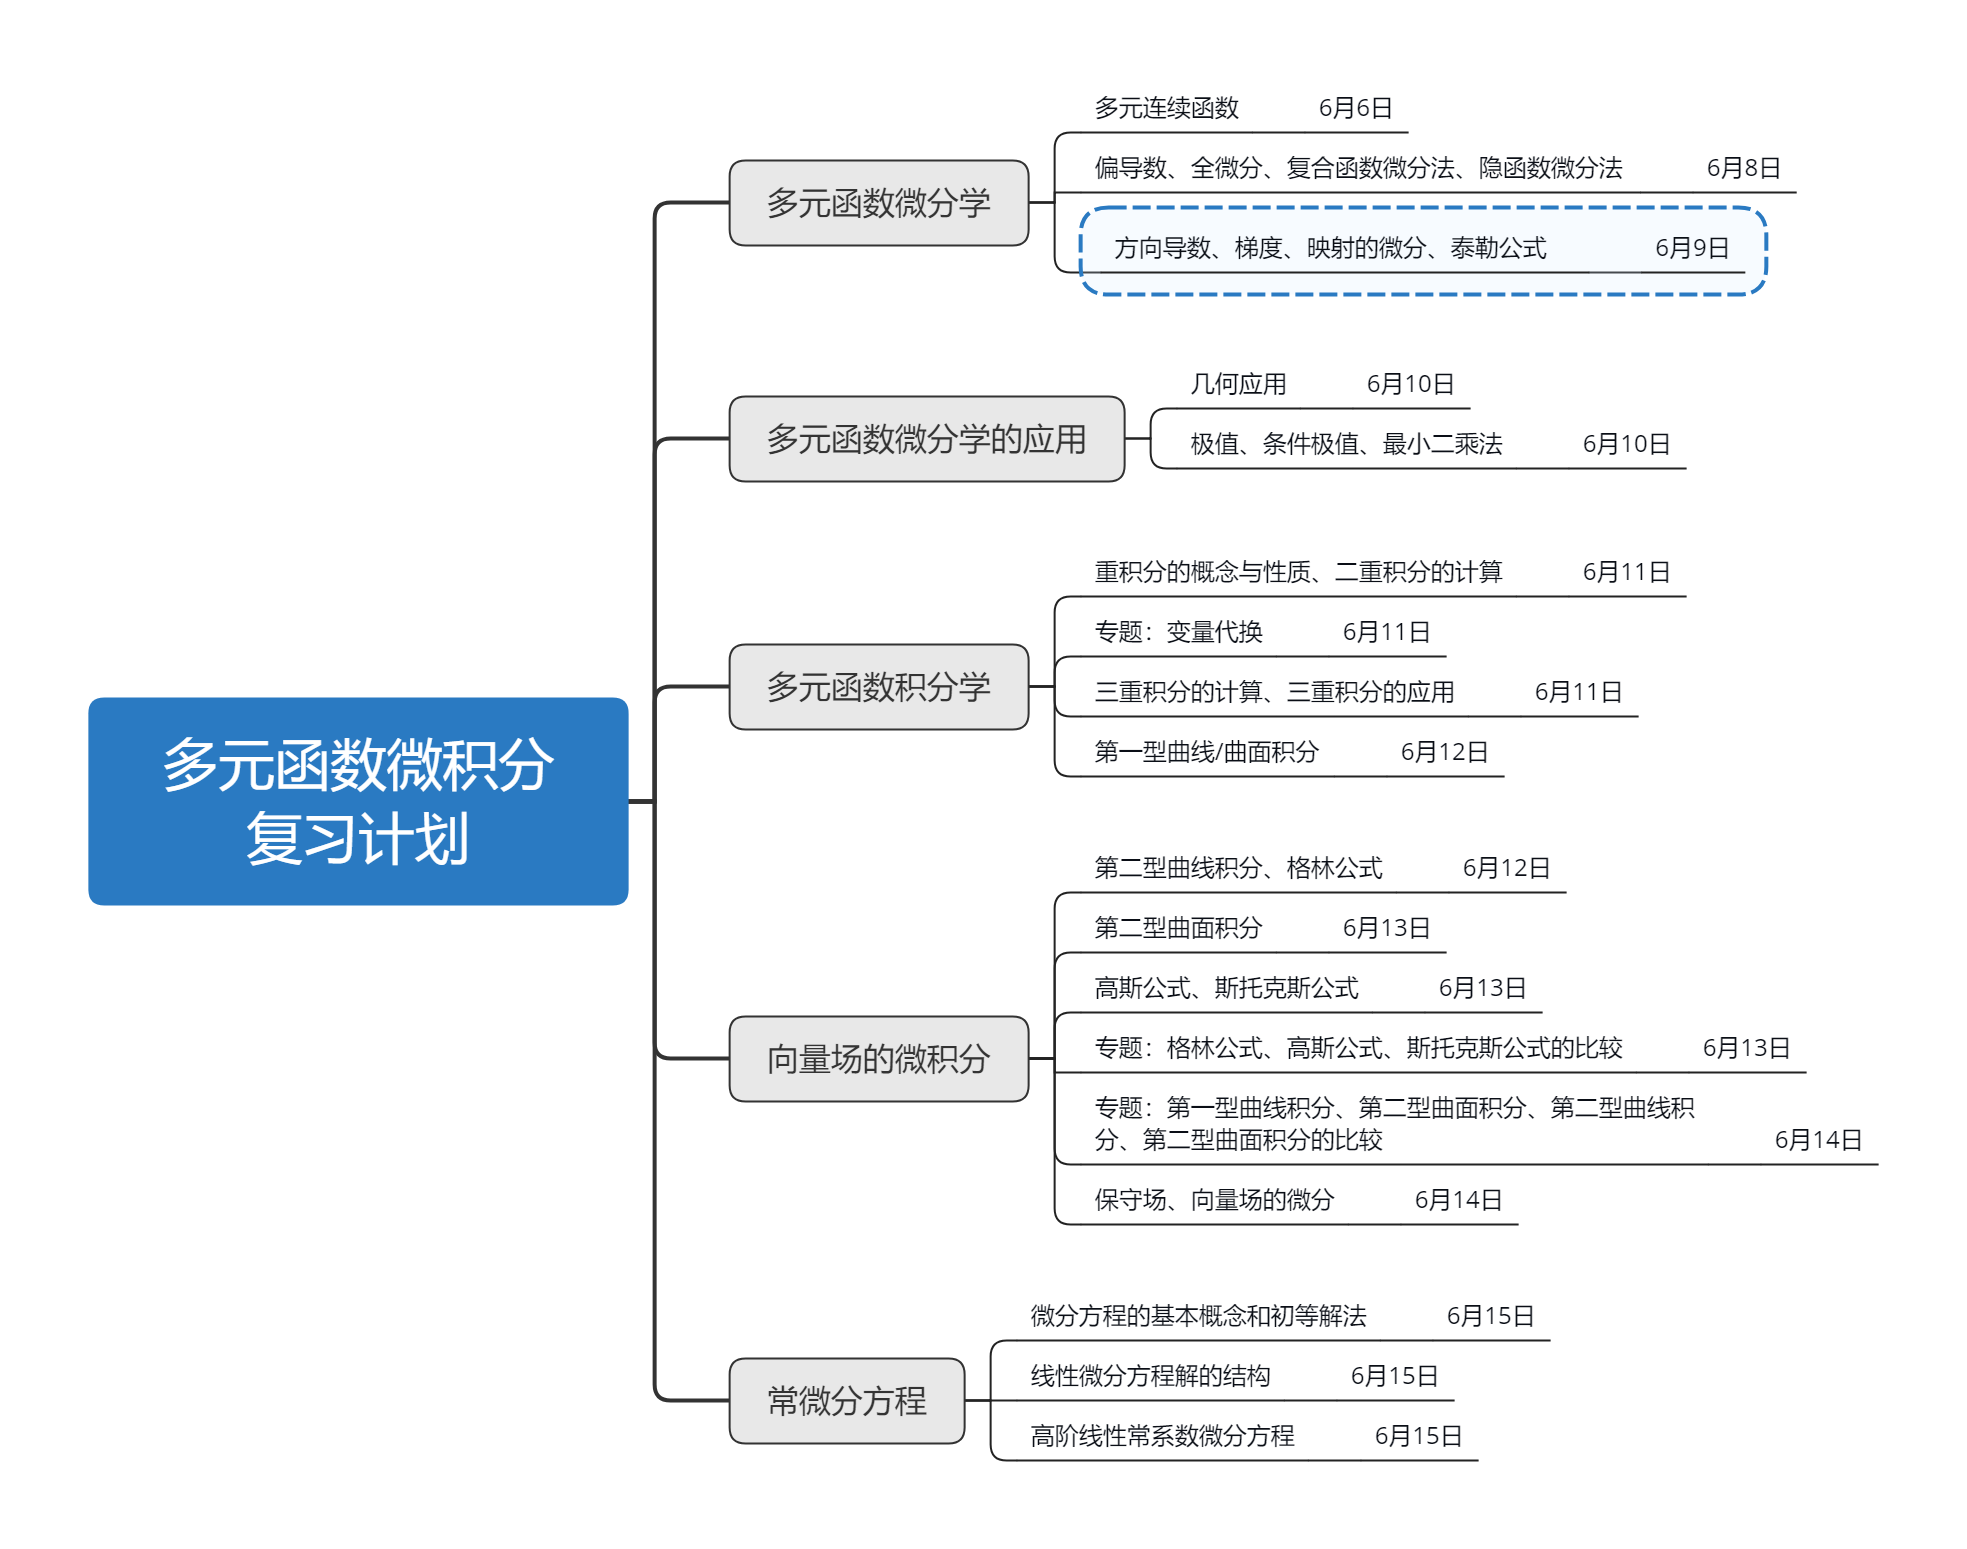
\includegraphics[height=0.5\textheight]{Figures20190609/plan.png}
\end{center}
\end{figure}
\subsection{知识结构}
\begin{figure}[H]
\begin{center}
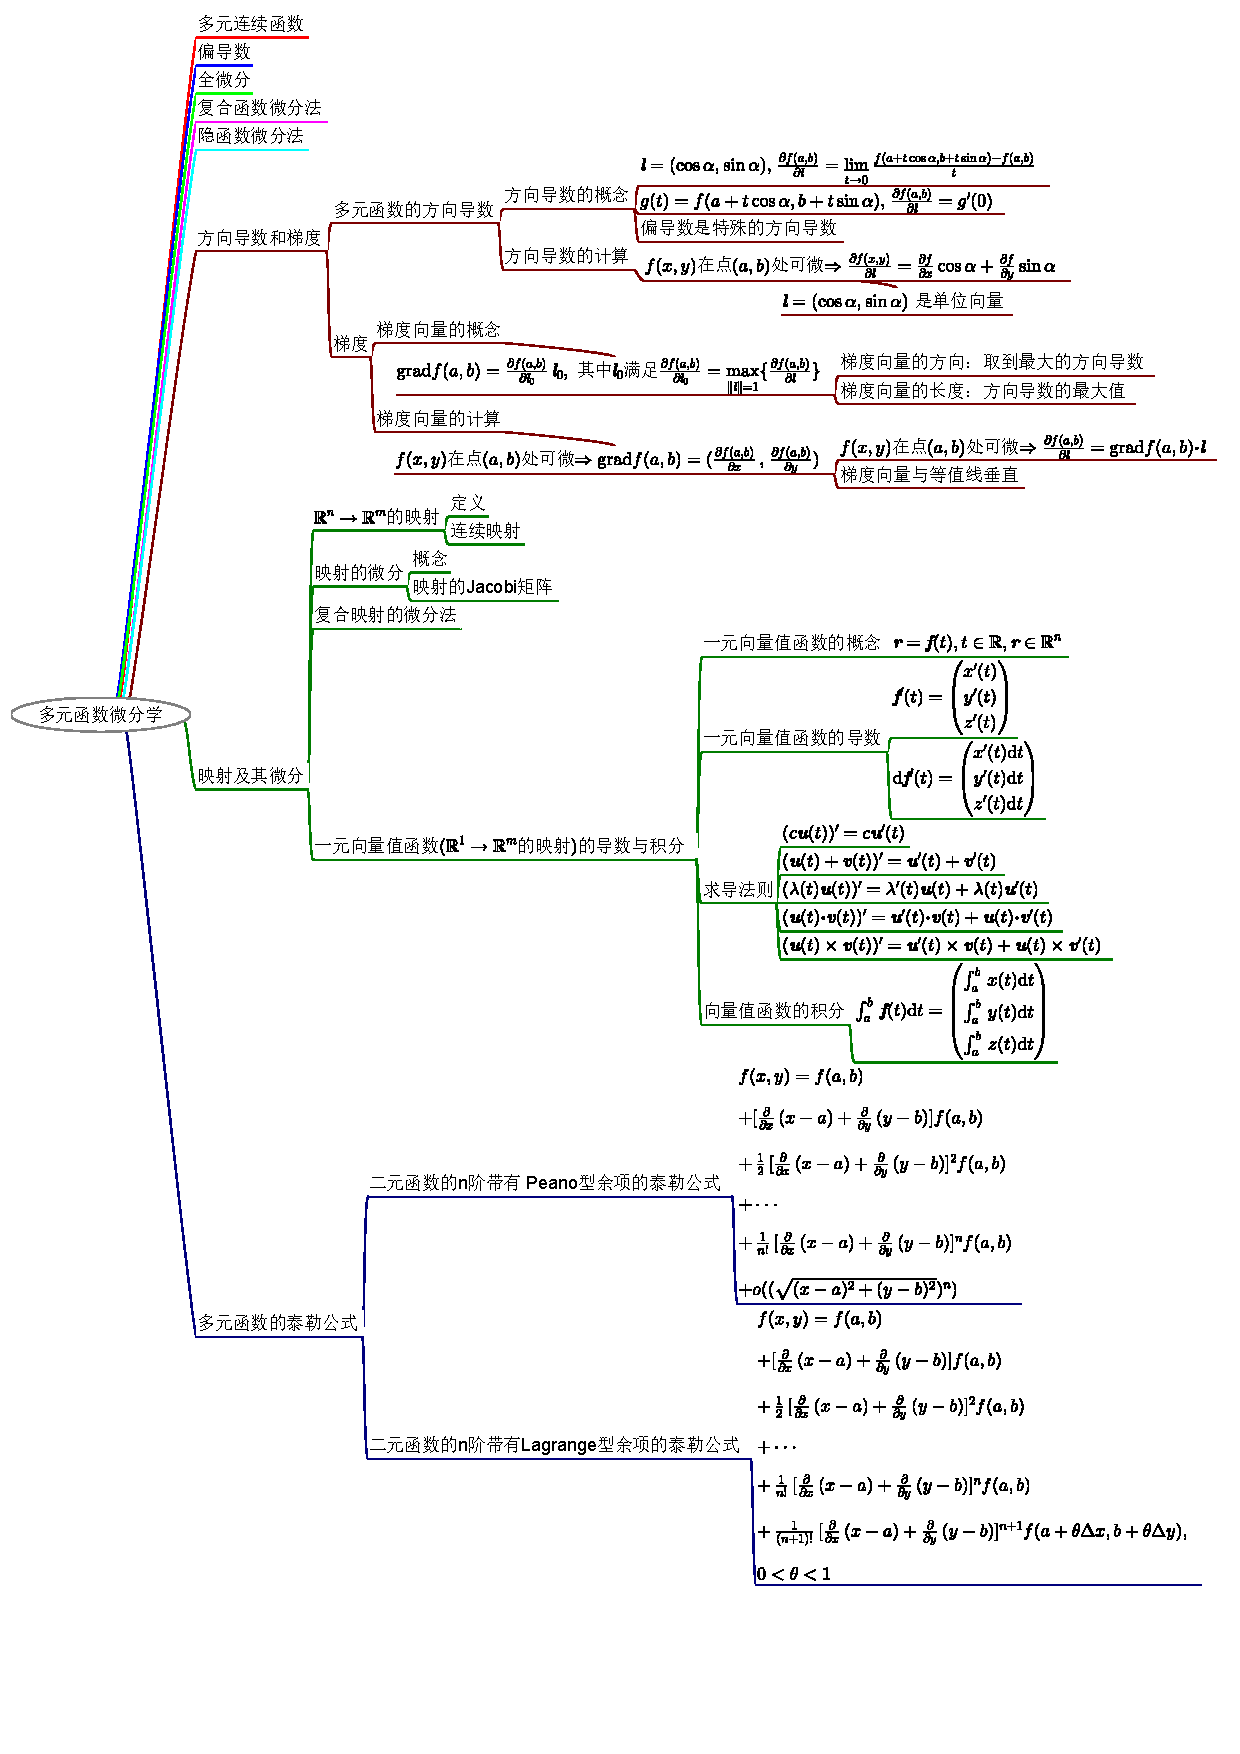
\includegraphics[height=0.9\textheight,angle=0]{20190609.pdf}
\end{center}
\end{figure}
\subsection{重要知识}
\begin{enumerate}
\item方向导数的几何意义.
\begin{figure}[H]
\begin{center}
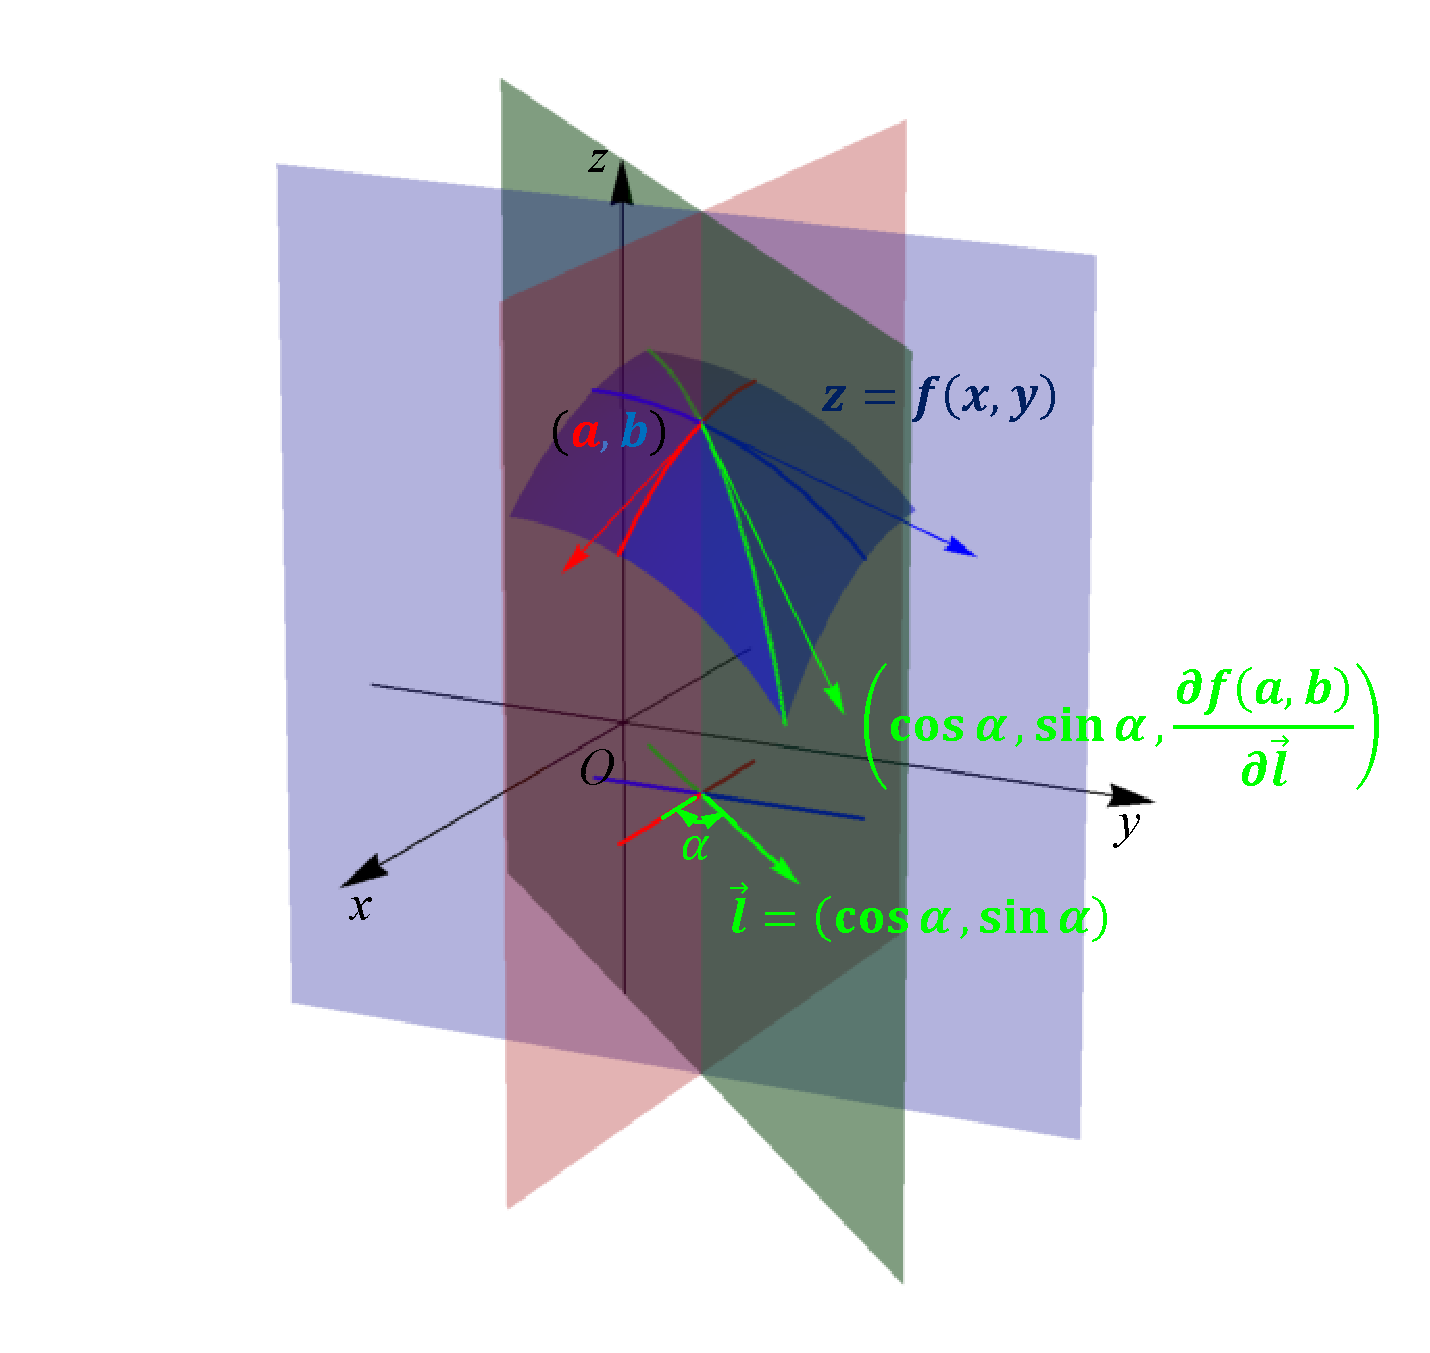
\includegraphics[height=0.6\textheight,angle=0]{Figures20190609/directedderivative.pdf}
\end{center}
\caption{方向导数的几何意义}
\end{figure}
\indent方向导数的几何意义如上图所示,须注意以下几点:
\begin{enumerate}
\item二元函数$f(x,y)$在一点处的方向导数$\frac{\partial f(a,b)}{\partial\bm l}$是函数在该点沿确定方向$\bm l=(\cos\alpha,\sin\alpha)$的变化率;
\item向量$(\cos\alpha,\sin\alpha,\frac{\partial f(a,b)}{\partial\bm l})$是函数$f(x,y)$在点$(a,b)$沿$\bm l$方向的切向量;
\item所有切向量的集合$\Set{\bm\tau}{\bm\tau=(\cos\alpha,\sin\alpha,\frac{\partial f(a,b)}{\partial\bm l}),\bm l=(\cos\alpha,\sin\alpha),\alpha\in[0,2\pi)}$共面;
\item偏导数是沿坐标轴{\bf正}方向的方向导数,
\item当函数$f(x,y)$在点$(a,b)$可微时,$\frac{\partial f(a,b)}{\partial\bm l}=\text{grad}f(a,b)\bm\cdot\bm l=\frac{\partial f(a,b)}{\partial x}\cos\alpha+\frac{\partial f(a,b)}{\partial y}\sin\alpha$.
\end{enumerate}
\item梯度的几何意义.
\begin{figure}[H]
\begin{center}
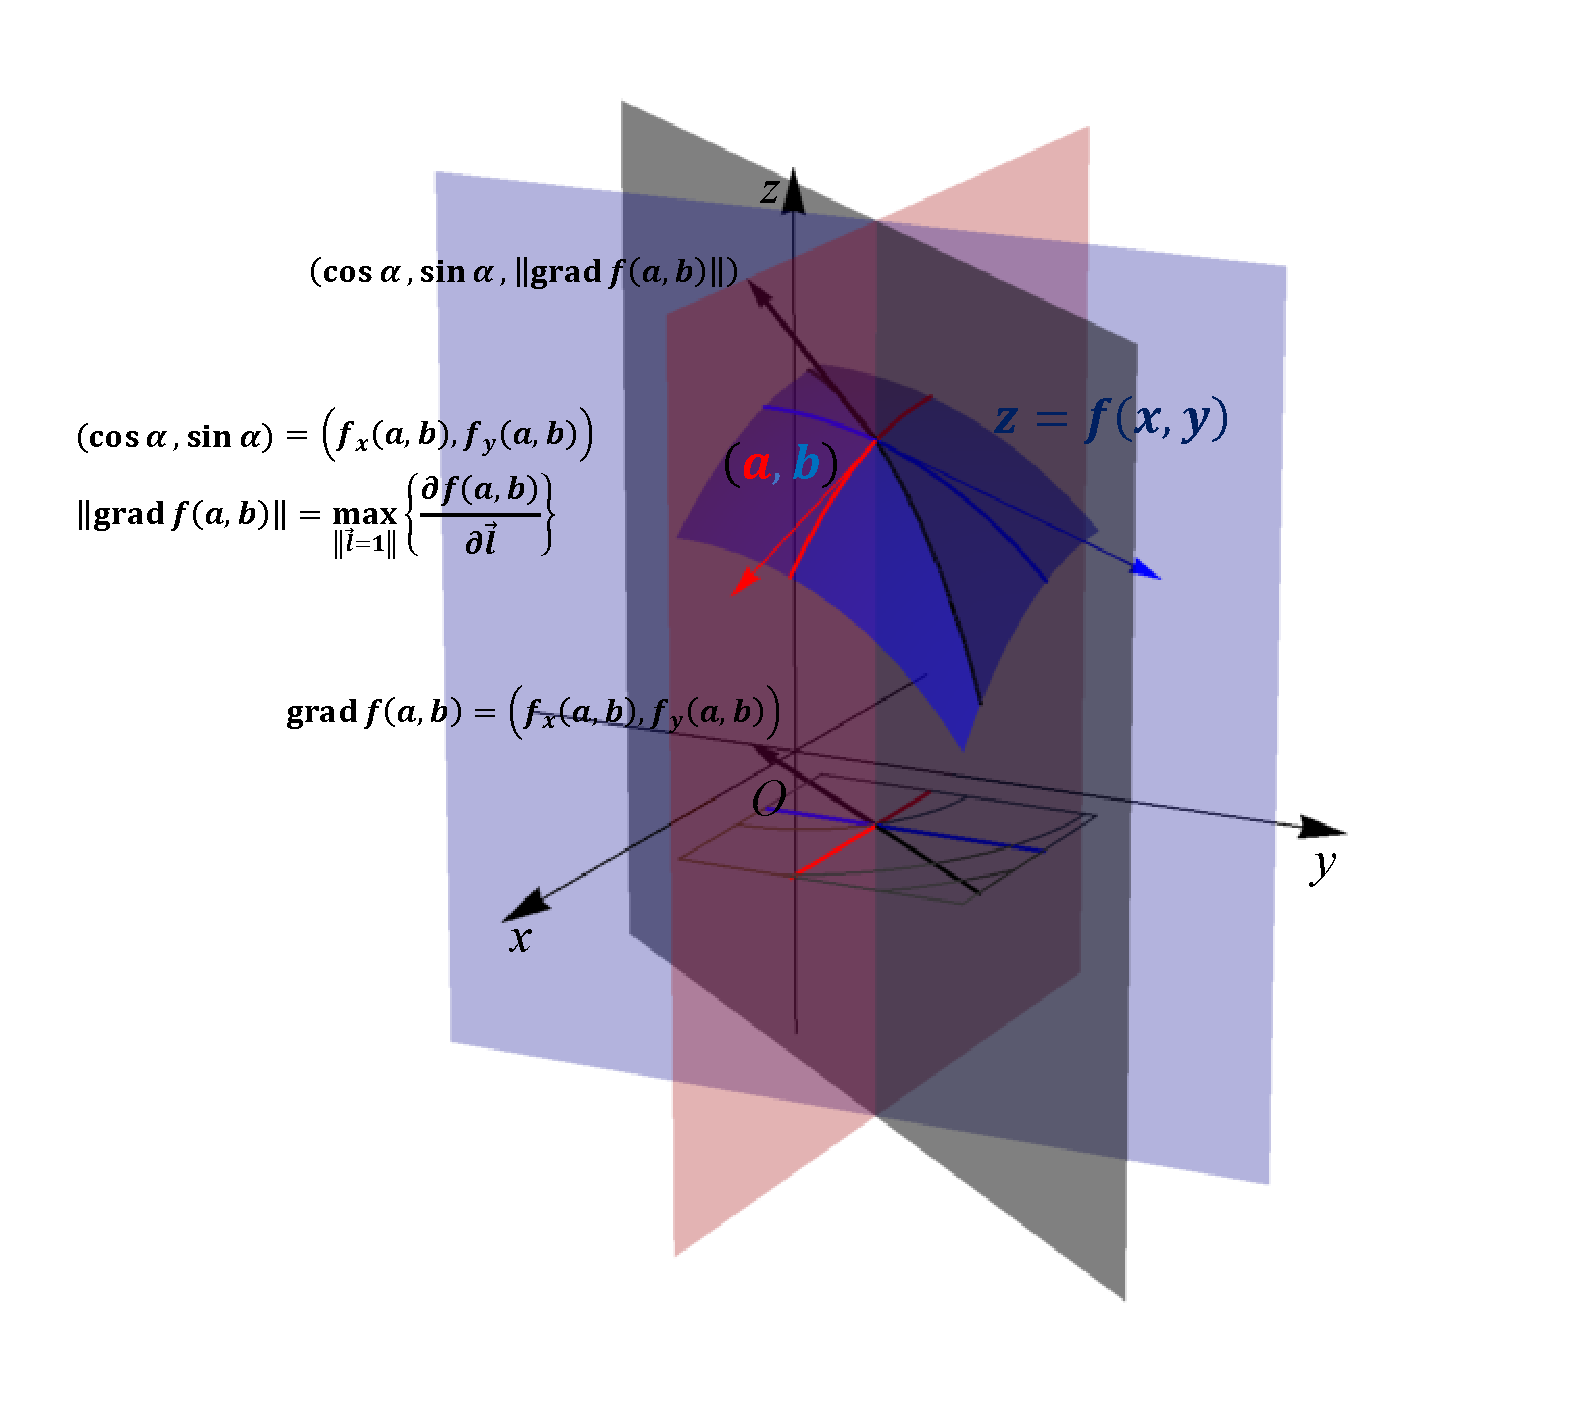
\includegraphics[height=0.6\textheight,angle=0]{Figures20190609/gradient.pdf}
\end{center}
\caption{梯度的几何意义}
\end{figure}
\indent梯度的几何意义如上图所示,须注意以下几点:
\begin{enumerate}
\item函数$f(x,y)$在点$(a,b)$处可微时,梯度$\text{grad}f(a,b)=(\frac{\partial f(a,b)}{\partial x},\frac{\partial f(a,b)}{\partial y})$;
\item梯度$\text{grad}f(a,b)$的方向为函数$f(x,y)$在点$(a,b)$处方向导数最大的方向;
\item因在一点$(a,b)$处的所有切向量的集合$\Set{\bm\tau}{\bm\tau=(\cos\alpha,\sin\alpha,\frac{\partial f(a,b)}{\partial\bm l}),\bm l=(\cos\alpha,\sin\alpha),\alpha\in[0,2\pi)}$共面,故最大的方向导数$\max\limits_{\alpha\in[0,2\pi)}\{\frac{f(a,b)}{\partial\bm l}\}$必为非负;
\item梯度向量的长度为方向导数的最大值,即$\|\text{grad}f(a,b)\|=\max\limits_{\alpha\in[0,2\pi)}\{\frac{f(a,b)}{\partial\bm l}\}$.
\end{enumerate}
\item可微与方向导数是否存在的关系.

函数$f(x,y)$在点$(a,b)$处可微,则函数$f(x,y)$在点$(a,b)$处的方向导数存在,但函数$f(x,y)$在点$(a,b)$处的方向导数存在时函数不一定可微.

反例1:函数$f(x,y)=\begin{cases}
1,&y=x^3,x\neq0,\\
0,&\text{otherwise},
\end{cases}$在点$(0,0)$沿任意方向的方向导数都存在,其值为$0$. 但函数$f(x,y)$在点$(0,0)$处不连续,故不可微. 此时$\frac{\partial f(a,b)}{\partial x}=0,\frac{\partial f(a,b)}{\partial y}=0$,方向导数$\frac{\partial f(x,y)}{\partial\bm l}=0=\frac{\partial f(a,b)}{\partial x}\cos\alpha+\frac{\partial f(a,b)}{\partial y}\sin\alpha$.

反例2:已知$f(x,y)=\begin{cases}
\frac{x^2y}{x^2+y^2},&x^2+y^2\neq0,\\
0,&x^2+y^2=0,
\end{cases}\bm l=(1,1)$,求$\frac{\partial f(0,0)}{\partial\bm l}$.

令$g(t)=f(\frac t{\sqrt 2},\frac t{\sqrt2})=\begin{cases}
\frac1{2\sqrt2}t,&t\neq0,\\
0,&t=0,
\end{cases}$,则$\frac{\partial f(0,0)}{\partial\bm l}=\frac1{2\sqrt2}$.

此时$\frac{\partial f(0,0)}{\partial x}=0,\frac{\partial f(0,0)}{\partial y}=0$,
若函数可微,则$\md f(0,0)=0$,
\[\lim\limits_{(x,y)\rightarrow(0,0)}\frac{\frac{x^2y}{x^2+y^2}-0-0}{\sqrt{x^2+y^2}}=\lim\limits_{(x,y)\rightarrow(0,0)}\frac{x^2y}{(x^2+y^2)^{\frac32}}=0.\]

但是$\lim\limits_{\substack{x\rightarrow0\\ y=kx}}\frac{kx^3}{(\sqrt{1+k^2})^3x^3}=\frac k{(1+k^2)^{\frac32}}$不恒等于0.

故$f(x,y)$在点$(0,0)$不可微.

此时$\frac{\partial f(0,0)}{\partial\bm l}=\frac1{2\sqrt2}\neq0=\frac{\partial f(a,b)}{\partial x}\cos\alpha+\frac{\partial f(a,b)}{\partial y}\sin\alpha$.
\end{enumerate}
\subsection{习题分类与解题思路}
\begin{enumerate}
\item方向导数与梯度
\begin{enumerate}
\item方向导数的计算,可用定义或者梯度进行计算. 当用梯度计算时,须注意在所求点上函数应可微,且应把方向向量单位化.

【如习题10.4中的5.】
\item考查梯度的几何意义. 

具体可见【习题10.4中的6.】
\end{enumerate}
\item一元向量值函数的导数与积分
\begin{enumerate}
\item考查向量值函数的四则运算法则.

【如习题11.1中的1., 2.】
\item求曲线的切向量或切线方程,即一元向量值函数的导数.

【如习题11.1中的2., 3., 7., 8.】
\item求一元向量值函数的积分.

【如习题11.1中的4., 9.】
\item已知一元向量值函数的导函数和定解条件,求原函数.

【如习题11.1中的5.】
\end{enumerate}
\item多元函数的泰勒公式
\begin{enumerate}
\item利用带佩亚诺余项的泰勒公式做近似计算.

【如习题10.6中的1.】
\item将函数展开成泰勒多项式.

【如习题10.6中的2.】
\item将函数展开成带拉格朗日余项的泰勒多项式.

【如习题10.6中的3.】
\end{enumerate}
\end{enumerate}
【第10章补充题的题目有一些综合性,大家可做一下积累.】
\subsection{习题10.4解答}
\begin{enumerate}
\item[5.]求$z=\ln(\mathrm e^{-x}+\frac{x^2}y)$在点$(1,1)$处沿$\bm v=(a,b)^T(a\neq0)$的方向导数.

解:$\because\frac{\partial z}{\partial x}=\frac{-\mathrm e^{-x}+\frac{2x}y}{\mathrm e^{-x}+\frac{x^2}y},\frac{\partial z}{\partial y}=\frac{-\frac{x^2}{y^2}}{\mathrm e^{-x}+\frac{x^2}y}$, 

$\therefore\mathrm{grad}z(1,1)=(\frac{\partial z(1,1)}{\partial x},\frac{\partial z(1,1)}{\partial y})=(\frac{-\mathrm e^{-1}+2}{\mathrm e^{-1}+1},\frac{-1}{\mathrm e^{-1}+1})=(\frac{2\mathrm e-1}{\mathrm e+1},-\frac{\mathrm e}{\mathrm e+1})$,

$\because\frac{\partial z}{\partial x},\frac{\partial z}{\partial y}$在点$(1,1)$及其附近存在且在点$(1,1)$处连续,

$\therefore f(x,y)$在点$(1,1)$处可微,

$\therefore\frac{\partial z(1,1)}{\partial\bm v}=\mathrm{grad}z(1,1)\cdot\frac{\bm v}{\|\bm v\|}=(\frac{2\mathrm e-1}{\mathrm e+1},-\frac{\mathrm e}{\mathrm e+1})\cdot\frac1{\sqrt{a^2+b^2}}(a,b)^T=\frac1{\sqrt{a^2+b^2}}(\frac{2a\mathrm e-a-b\mathrm e}{\mathrm e+1})$.

\item[6.]已知$f(x,y)=x^2-xy+y^2$.\\
(1)当$\bm v$分别为何向量时,方向导数$\frac{\partial f(1,1)}{\partial\bm v}$会取到最大值、最小值和零值?并求出其最大值和最小值.\\
(2)试求$\mathrm{grad}f(1,1)$,并说明其方向与大小的意义.

解:(1)$\because\frac{\partial f(x,y)}{\partial x}=2x-y,\frac{\partial f(x,y)}{\partial y}=2y-x$,

$\therefore\mathrm{grad}f(1,1)=(\frac{\partial f(1,1)}{\partial x},\frac{\partial f(1,1)}{\partial y})=(1,1)$,

$\because\frac{\partial z}{\partial x},\frac{\partial z}{\partial y}$在点$(1,1)$及其附近存在且在点$(1,1)$处连续,

$\therefore f(x,y)$在点$(1,1)$处可微,

$\therefore\frac{\partial f(1,1)}{\partial\bm v}=\mathrm{grad}f(1,1)\cdot\bm v=\|\mathrm{grad}f(1,1)\|\|\bm v\|\cos\theta=\|\mathrm{grad}f(1,1)\|\cos\theta$,

当$\bm v$与梯度向量的夹角$\theta=0$即$\bm v=\frac1{\sqrt2}(1,1)$时,方向导数$\frac{\partial f(1,1)}{\partial\bm v}$取得最大值$\|\mathrm{grad}f(1,1)\|=\sqrt2$;

当$\bm v$与梯度向量的夹角$\theta=\pi$即$\bm v=-\frac1{\sqrt2}(1,1)$时,方向导数$\frac{\partial f(1,1)}{\partial\bm v}$取得最小值$-\|\mathrm{grad}f(1,1)\|=-\sqrt2$;

当$\bm v$与梯度向量的夹角$\theta=\frac\pi2$即$\bm v=\frac1{\sqrt2}(-1,1)$或$\frac1{\sqrt2}(1,-1)$时,方向导数$\frac{\partial f(1,1)}{\partial\bm v}=0$.

(2)$\mathrm{grad}f(1,1)=(1,1)$,其方向表示方向导数最大的方向,其大小为方向导数的最大值.
\end{enumerate}
\subsection{习题10.6解答}
\begin{enumerate}
\item写出$f(x,y)=x^y$在点$(1,1)$带佩亚诺余项的三阶泰勒公式,由此计算$1.1^{1.02}$.

解:$f(1,1)=1$,

$\frac{\partial f}{\partial x}=yx^{y-1},\frac{\partial f}{\partial y}=x^y\ln x$,

$\frac{\partial^2f}{\partial x^2}=y(y-1)x^{y-2},\frac{\partial^2f}{\partial x\partial y}=x^{y-1}+yx^{y-1}\ln x,\frac{\partial^2f}{\partial y^2}=x^y(\ln x)^2$,

$\frac{\partial^3f}{\partial x^3}=y(y-1)(y-2)x^{y-3},\frac{\partial^3f}{\partial x\partial y^2}=yx^{y-1}(\ln x)^2,\\
\frac{\partial^3}{\partial y\partial x^2}=(2y-1)x^{y-2}+y(y-1)x^{y-2}\ln x=[(2y-1)+y(y-1)\ln x]x^{y-2},\\
\frac{\partial^3f}{\partial y^3}=x^y(\ln x)^3$,

$\therefore$
\[\begin{split}
&f(x,y)\\
=&f(1,1)+[\frac{\partial f(1,1)}{\partial x}(x-1)+\frac{\partial f(1,1)}{\partial y}(y-1)]\\
&+\frac12[\frac{\partial^2f(1,1)}{\partial x^2}(x-1)^2+2\frac{\partial^2f(1,1)}{\partial x\partial y}(x-1)(y-1)+\frac{\partial^2f(1,1)}{\partial y^2}(y-1)^2]\\
&+\frac16[\frac{\partial^3f(1,1)}{\partial x^3}(x-1)^3+3\frac{\partial^3f(1,1)}{\partial x\partial y^2}(x-1)(y-1)^2+3\frac{\partial^3f(1,1)}{\partial y\partial x^2}(x-1)^2(y-1)\\
&\hspace{7cm}+\frac{\partial^3f(1,1)}{\partial y^3}(y-1)^3]+o[(\sqrt{(x-1)^2+(y-1)^2})^3]\\
=&1+(x-1)+\frac12[2(x-1)(y-1)]+\frac16[3(x-1)^2(y-1)]+o[(\sqrt{(x-1)^2+(y-1)^2})^3]\\
=&x+(x-1)(y-1)+\frac12(x-1)^2(y-1)+o[(\sqrt{(x-1)^2+(y-1)^2})^3]
\end{split}\]

$\therefore1.1^{1.02}=f(1.1,1.02)\approx1+0.1+0.1\times0.02+\frac12\times0.1^2\times0.02=1.1021$.

\item证明当$|x|,|y|$充分小时,有$\frac{\cos x}{\cos y}\approx1-\frac12(x^2-y^2)$.

证明:记$f(x,y)=\frac{\cos x}{\cos y}$,

$f(0,0)=1$,
\begin{flalign*}
&\frac{\partial f}{\partial x}=-\frac{\sin x}{\cos y},\frac{\partial f}{\partial y}=\frac{\cos x\sin y}{\cos^2y},\\
&\frac{\partial^2f}{\partial x^2}=-\frac{\cos x}{\cos y},\frac{\partial^2f}{\partial x\partial y}=-\frac{\sin x\sin y}{\cos^2y},\\
&\frac{\partial^2f}{\partial y^2}=\frac{\cos x\cos y\cos^2y+\cos x\sin y2\cos y\sin y}{\cos^4y}=\frac{\cos x\cos^2y+2\cos x\sin^2y}{\cos^3y},&
\end{flalign*}
$\therefore$
\[\begin{split}
f(x,y)=&f(0,0)+[\frac{\partial f(0,0)}{\partial x}x+\frac{\partial f(0,0)}{\partial y}y]+\frac12[\frac{\partial^2f(0,0)}{\partial x^2}x^2+2\frac{\partial^2f(0,0)}{\partial x\partial y}xy+\frac{\partial^2f(0,0)}{\partial y^2}y^2]\\
&+o[(\sqrt{x^2+y^2})^2]\\
=&1+(0+0)+\frac12(-x^2+0+y^2)+o[(\sqrt{x^2+y^2})^2]\\
=&1-\frac12(x^2-y^2)+o[(\sqrt{x^2+y^2})^2],
\end{split}\]
$\therefore$当$|x|,|y|$充分小时,有$\frac{\cos x}{\cos y}\approx1-\frac12(x^2-y^2)$.

\item写出$f(x,y)=\sqrt{1+y^2}\cos x$在点$(0,1)$的一阶泰勒多项式及拉格朗日余项.

解:$f(0,1)=\sqrt2$,
\begin{flalign*}
&\frac{\partial f}{\partial x}=-\sqrt{1+y^2}\sin x,\frac{\partial f}{\partial y}=\frac{2y\cos x}{2\sqrt{1+y^2}}=\frac{y\cos x}{\sqrt{1+y^2}},\\
&\frac{\partial^2f}{\partial x^2}=-\sqrt{1+y^2}\cos x,\frac{\partial^2f}{\partial x\partial y}=\frac{-2y\sin x}{2\sqrt{1+y^2}}=\frac{-y\sin x}{\sqrt{1+y^2}},\\
&\frac{\partial^2f}{\partial y^2}=\frac{\cos x\sqrt{1+y^2}-y\cos x\frac{2y}{2\sqrt{1+y^2}}}{1+y^2}=\frac{\cos x}{(1+y^2)^{\frac32}},&
\end{flalign*}
$\therefore$
\[\begin{split}
f(x,y)=&f(0,1)+[\frac{\partial f(0,1)}{\partial x}x+\frac{\partial f}{\partial y}(y-1)]\\
&+\frac12[\frac{\partial^2f(\theta x,1+\theta(y-1))}{\partial x^2}x^2+2\frac{\partial^2f(\theta x,1+\theta(y-1))}{\partial x\partial y}x(y-1)\\
&\hspace{7cm}+\frac{\partial^2f(\theta x,1+\theta(y-1))}{\partial y^2}(y-1)^2]\\
=&\sqrt2+\frac{\sqrt2}2(y-1)\\
&+\frac12\Big(-\sqrt{1+[1+\theta(y-1)]^2}\cos(\theta x)x^2-\frac{2[1+\theta(y-1)]\sin\theta x}{\sqrt{1+[1+\theta(y-1)]^2}}x(y-1)\\
&\hspace{7cm}+\frac{\cos\theta x}{\{1+[1+\theta(y-1)]^2\}^{\frac32}}(y-1)^2\Big)\\
=&\sqrt2+\frac{\sqrt2}2(y-1)\\
&+\frac12\Big\{-x^2\sqrt{1+(1+\theta(y-1))^2}\cos\theta x-2x(y-1)\frac{1+\theta(y-1)}{\sqrt{1+(1+\theta(y-1))^2}}\sin\theta x\\
&\hspace{6cm}+(y-1)^2\frac{\cos\theta x}{\{1+(1+\theta(y-1))^2\}^{\frac32}}\Big\},0<\theta<1.
\end{split}\]
\end{enumerate}
\subsection{第10章补充题}
\begin{enumerate}
\item设$f(x,y)$是定义在整个平面上的连续函数,当$x^2+y^2\rightarrow+\infty$时,$f(x,y)\rightarrow+\infty$. 求证存在$(x_0,y_0)$,使
\[
f(x_0,y_0)=\min\Set{f(x,y)}{(x,y)\in\mathbb R^2}.
\]
证明:$\because$当$x^2+y^2\rightarrow+\infty$时,$f(x,y)\rightarrow+\infty$,

$\therefore$对于$f(0,0),\exists N>0,s.t.f(x,y)>f(0,0),x^2+y^2>N^2$,

$\because$在有界闭区域$D=\Set{(x,y)}{x^2+y^2\leq N^2}$内部$f(x,y)$连续,

$\therefore\exists(x_0,y_0)\in D,s.t.f(x_0,y_0)\leq f(x,y),(x,y)\in D$,此时$f(x_0,y_0)\leq f(0,0)$,

$\therefore f(x_0,y_0)\leq f(0,0)<f(x,y),x^2+y^2>N^2$,

$\therefore f(x_0,y_0)\leq f(x,y),(x,y)\in\mathbb R^2$,

$\therefore$存在$(x_0,y_0)$,使$f(x_0,y_0)=\min\Set{f(x,y)}{(x,y)\in\mathbb R^2}$.
\item设$f(x,y)$是定义在整个平面上的连续函数,$f(0,0)=0$,且当$(x,y)\neq(0,0)$时,$f(x,y)>0$,又设对于任意的$(x,y)$和任意实数$c$,都有
\[
f(cx,cy)=c^2f(x,y).
\]
求证存在正数$a,b$,使得对于任意的$(x,y)$,都有
\[
a(x^2+y^2)\leq f(x,y)\leq b(x^2+y^2).
\]
证明:$\because f(x,y)$是定义在整个平面上的连续函数,

$\therefore f(x,y)$在有界闭区域$D=\Set{(x,y)}{0.5<x^2+y^2\leq 1.5}$上连续,

$\because$当$(x,y)\neq(0,0)$时,$f(x,y)>0$,

$\therefore\exists b\geq a>0,s.t.a\leq f(x,y)\leq b,(x,y)\in D$,

$\therefore$当$(x,y)\in D^*=\Set{(x,y)}{x^2+y^2=1}\subset D$时,$a\leq f(x,y)\leq b$,

$\because f(x,y)=f(\sqrt{x^2+y^2}\frac x{\sqrt{x^2+y^2}},\sqrt{x^2+y^2}\frac y{x^2+y^2})=(x^2+y^2)f(\frac x{\sqrt{x^2+y^2}},\frac y{\sqrt{x^2+y^2}})$,

又$\because a\leq f(\frac x{\sqrt{x^2+y^2}},\frac y{\sqrt{x^2+y^2}})\leq b$,

$\therefore a(x^2+y^2)\leq f(x,y)\leq b(x^2+y^2)$.

\item若对于任意实数$t$,函数$f(x,y,z)$满足$f(tx,ty,tz)=t^kf(x,y,z)$,则称$f(x,y,z)$为$k$次齐次函数. 试证$k$次齐次函数$f(x,y,z)$满足方程
\[
x\frac{\partial f}{\partial x}+y\frac{\partial f}{\partial y}+z\frac{\partial f}{\partial z}=kf(x,y,z).
\]
证明:方法1:等式$f(tx,ty,tz)=t^kf(x,y,z)$两边分别对$t$求偏导得
\[
x\frac{\partial f(tx,ty,tz)}{\partial x}+y\frac{\partial f(tx,ty,tz)}{\partial y}+z\frac{\partial f(tx,ty,tz)}{\partial z}=kt^{k-1}f(x,y,z),
\]
令$t=1$得
\[
x\frac{\partial f}{\partial x}+y\frac{\partial f}{\partial y}+z\frac{\partial f}{\partial z}=kf(x,y,z).
\]

方法2:$\because f(tx,ty,tz)=t^kf(x,y,z)$,

$\therefore$
\begin{subequations}
\begin{align}
\frac{\partial f(x,y,z)}{\partial x}=\frac{\partial}{\partial x}\frac{f(tx,ty,tz)}{t^k}=\frac1{t^k}\frac{\partial f(tx,ty,tz)}{\partial x}t=\frac1{t^{k-1}}\frac{\partial f(tx,ty,tz)}{\partial x},\label{3a}\\
\frac{\partial f(x,y,z)}{\partial y}=\frac{\partial}{\partial y}\frac{f(tx,ty,tz)}{t^k}=\frac1{t^k}\frac{\partial f(tx,ty,tz)}{\partial y}t=\frac1{t^{k-1}}\frac{\partial f(tx,ty,tz)}{\partial y},\label{3b}\\
\frac{\partial f(x,y,z)}{\partial z}=\frac{\partial}{\partial z}\frac{f(tx,ty,tz)}{t^k}=\frac1{t^k}\frac{\partial f(tx,ty,tz)}{\partial z}t=\frac1{t^{k-1}}\frac{\partial f(tx,ty,tz)}{\partial z},\label{3c}
\end{align}
\end{subequations}
方程$f(tx,ty,tz)=t^kf(x,y,z)$两边分别对$t$求导
\[
x\frac{\partial f(tx,ty,tz)}{\partial x}+y\frac{\partial f(tx,ty,tz)}{\partial y}+z\frac{\partial f(tx,ty,tz)}{\partial z}=kt^{k-1}f(x,y,z),
\]
将式~(\ref{3a})-(\ref{3c})代入上式
\[
xt^{k-1}\frac{\partial f(x,y,z)}{\partial x}+yt^{k-1}\frac{\partial f(x,y,z)}{\partial y}+zt^{k-1}\frac{\partial f(x,y,z)}{\partial z}=kt^{k-1}f(x,y,z),
\]
即
\[
x\frac{\partial f}{\partial x}+y\frac{\partial f}{\partial y}+z\frac{\partial f}{\partial z}=kf(x,y,z).
\]
\item设$F$为三元可微函数,$u=u(x,y,z)$是由方程$F(u^2-x^2,u^2-y^2,u^2-z^2)=0$确定的隐函数. 求证
\[
\frac{u'_x}{x}+\frac{u'_y}{y}+\frac{u'_z}{z}=\frac1u.
\]
证明:方程$F(u^2-x^2,u^2-y^2,u^2-z^2)=0$两边分别对$x$求偏导
\[
F'_1(2u\frac{\partial u}{\partial x}-2x)+F'_22u\frac{\partial u}{\partial x}+F'_32u\frac{\partial u}{\partial x}=0
\]
得
\[
\frac{\partial u}{\partial x}=\frac{xF'_1}{u(F'_1+F'_2+F'_3)}
\]
同理
\[\begin{split}
\frac{\partial u}{\partial y}=\frac{yF'_2}{u(F'_1+F'_2+F'_3)},\\
\frac{\partial u}{\partial z}=\frac{zF'_3}{u(F'_1+F'_2+F'_3)},
\end{split}\]
$\therefore$
\[
\frac{u'_x}{x}+\frac{u'_y}{y}+\frac{u'_z}{z}=\frac{F'_1+F'_2+F'_3}{u(F'_1+F'_2+F'_3)}=\frac1u.
\]
\item求方程$\frac{\partial^2z}{\partial x\partial y}=x+y$满足条件$z(x,0)=x,z(0,y)=y^2$的解$z(z,y)$.

解:方法1:$\because\frac{\partial^2z}{\partial x\partial y}=x+y$,

$\therefore\frac{\partial z}{\partial y}=\int_0^x(x+y)\mathrm dx+\varphi_0(y)=\frac{x^2}2+xy+\varphi_0(y)$,

$\because z(0,y)=y^2$,

$\therefore\frac{z(0,y)}{\partial y}=2y=\varphi_0(y)$,

$\therefore z(x,y)=\int_0^y[\frac{x^2}2+xy+2y]\mathrm dy+\psi(x)=\frac12x^2y+\frac12xy^2+y^2+\psi(x)$,

$\because z(x,0)=x=\psi(x)$,

$\therefore z(x,y)=\frac12x^2y+\frac12xy^2+y^2+x$.

方法2:$\because\frac{\partial^2z}{\partial x\partial y}=x+y$,

$\therefore\int\frac{\partial^2z}{\partial x\partial y}\mathrm dx=\int(x+y)\mathrm dx=\frac12x^2+xy+C_1(y)=\frac{\partial z}{\partial y}+C_1(y)$,

$\therefore$可设$\frac{\partial z}{\partial y}=\frac12x^2+xy+C(y)$,其中$C(y)$是与$x$无关的$y$的函数,

$\because z(0,y)=y^2$,

$\therefore\frac{\partial z(0,y)}{\partial y}=2y=C(y)$,

$\therefore\frac{\partial z}{\partial y}=\frac12x^2+xy+2y$,

$\therefore\int\frac{\partial z}{\partial y}\mathrm dy=\int(\frac12x^2+xy+2y)\mathrm dy=\frac12x^2y+\frac12xy^2+y^2+C_3(x)=z(x,y)+C_4(x)$,

$\therefore$可设$z(x,y)=\int(\frac12x^2+xy+2y)\mathrm dy+C^*(x)=\frac12x^2y+\frac12xy^2+y^2+C^*(x)$,其中$C^*(x)$是与$y$无关的$x$的函数,

$\because z(x,0)=x=C^*(x)$,

$\therefore z(x,y)=\frac12x^2y+\frac12xy^2+y^2+x$.

方法3:$\because\frac{\partial^2z}{\partial x\partial y}=x+y$,

$\therefore\int\frac{\partial^2z}{\partial x\partial y}\mathrm dx=\int(x+y)\mathrm dx=\frac12x^2+xy+C_1(y)=\frac{\partial z}{\partial y}+C_2(y)$,

$\therefore$可设$\frac{\partial z}{\partial y}=\frac12x^2+xy+C(y)$,其中$C(y)$是与$x$无关的$y$的函数,

$\therefore\int\frac{\partial z}{\partial y}\mathrm dy=\frac12x^2y+\frac12xy^2+\int C(y)\mathrm dy=z(x,y)+C_3(x)$,

$\therefore$可设$z(x,y)=\frac12x^2y+\frac12xy^2+F(y)+C^*(x)$,其中$F(y)$是$C(y)$的一个与$x$无关的原函数,$C^*(x)$是与$y$无关的$x$的函数,

$\because z(0,y)=y^2,z(x,0)=x$,

$\therefore F(y)+C^*(0)=y^2,F(0)+C^*(x)=x$,

$\therefore F(y)=y^2-C^*(0),C^*(x)=x-F(0)$,且$F(0)+C^*(0)=0$,

$\therefore z(x,y)=\frac12x^2y+\frac12xy^2+y^2+x-[F(0)+C^*(0)]=\frac12x^2y+\frac12xy^2+y^2+x$.
\item设$z=f(x,y)$处处可微,$a,b$不全等于零. 求证满足方程$bz'_x=az'_y$的充分条件是存在一元函数$g(u)$,使得$z=f(x,y)=g(ax+by)$.

证明:$\because$存在一元函数$g(u)$,使得$z=f(x,y)=g(ax+by)$,

$\therefore$对于任意常数$C$,$z$在直线$ax+by=C$上恒等于常数,

$\therefore z=f(x,y)$在直线$ax+by=C$上任意一点处沿该直线方向的方向导数均等于零,

由$a,b$不全为零知直线$ax+by=C$的方向向量可表示为$(-b,a)$,

又$\because z=f(x,y)$处处可微,

$\therefore z=f(x,y)$在直线$ax+by=C$上的每一点处沿$(-b,a)$方向的方向导数
\[\frac{\partial z}{\partial\bm l}=\mathrm{grad}z\bm\cdot\frac1{a^2+b^2}(-b,a)=(z'_x,z'_y)\bm\cdot\frac1{a^2+b^2}(-b,a)=\frac1{\sqrt{a^2+b^2}}(-bz'_x+az'_y)=0,\]
$\therefore$在直线$ax+by=C$上的每一点处$bz'_x=az'_y$,由$C$的任意性知$bz'_x=az'_y$处处成立.

\item设$D$为包含原点$O(0,0)$的一个圆域. $f(x,y)$在$D$中处处有连续偏导数,并且满足$xf'_x+yf'_y=0$. 求证$f(x,y)$在$D$中恒等于某个常数.

证明:$\because f(x,y)$在$D$中处处有连续偏导数,

$\therefore f(x,y)$在$D$中处处可微,

$\therefore f(x,y)$在点$(x,y)\in D((x,y)\neq(0,0))$处由原点$(0,0)$指向点$(x,y)$方向的方向导数
\[\frac{\partial f(x,y)}{\partial\bm v}=\mathrm{grad}f(x,y)\bm\cdot\frac1{\sqrt{x^2+y^2}}(x,y)=\frac1{\sqrt{x^2+y^2}}(f'_x,f'_y)\bm\cdot(x,y)=\frac{xf'_x+yf'_y}{\sqrt{x^2+y^2}}=0,\]
$\therefore f(x,y)$在$D$中由原点出发且不含原点的每一条射线上任一点处沿该射线方向的方向导数均为$0$,

$\therefore f(x,y)$在$D$中由原点出发且不含原点的每一条射线上均为常数,

$\because f(x,y)$在$D$中处处可微,故处处连续,故在原点$(0,0)$处连续,

$\therefore f(x,y)$在$D$中由原点出发的每一条射线上均等于$f(0,0)$,

$\therefore f(x,y)=f(0,0),(x,y)\in D$.
%
%【注意:】如果区域$D$不包含原点,但仍有$f(x,y)$在$D$中处处有连续偏导数,并且满足$xf'_x+yf'_y=0$. 则$f(x,y)$在$D$中不一定恒等于常数,比如函数
%\[f(x,y)=
%\begin{cases}
%\cos(\arccos\frac x{\sqrt{x^2+y^2}}),&y\geqslant0,\\
%\cos(2\pi-\arccos\frac x{\sqrt{x^2+y^2}}),&y<0,
%\end{cases}\]
%该函数在极坐标下的方程是$f(r\cos\theta,r\sin\theta)=\cos\theta$,函数$f(x,y)$在$D$中处处有连续偏导数,且在由原点出发的每一条射线$\theta=C$上均为常数$\cos C$,故满足$xf'_x+yf'_y=0$,但$f(x,y)\not\equiv const$.
%
%\item[7.]设$D$为包含原点$O(0,0)$的一个圆域. $f(x,y)$在$D$中处处有连续偏导数,并且满足$xf'_x+yf'_y=0$. 求证$f(x,y)$在$D$中恒等于某个常数.
%
%证明:$\because f(x,y)$在$D$中处处有连续偏导数,
%
%$\therefore f(x,y)$在$D$中处处可微,
%
%$\therefore f(x,y)$在点$(x,y)\in D((x,y)\neq(0,0))$处由原点$(0,0)$指向点$(x,y)$方向的方向导数
%\[\frac{\partial f(x,y)}{\partial\bm v}=\mathrm{grad}f(x,y)\bm\cdot\frac1{\sqrt{x^2+y^2}}(x,y)=\frac1{\sqrt{x^2+y^2}}(f'_x,f'_y)\bm\cdot(x,y)=\frac{xf'_x+yf'_y}{\sqrt{x^2+y^2}}=0,\]
%$\therefore f(x,y)$在$D$中由原点出发且不含原点的每一条射线上任一点处沿该射线方向的方向导数均为$0$,
%
%$\therefore f(x,y)$在$D$中由原点出发且不含原点的每一条射线上均为常数,
%
%$\because f(x,y)$在$D$中处处可微,故处处连续,故在原点$(0,0)$处连续,
%
%$\therefore f(x,y)$在$D$中由原点出发的每一条射线上均等于$f(0,0)$,
%
%$\therefore f(x,y)=f(0,0),(x,y)\in D$.

【注意:】如果区域$D$不包含原点,但仍有$f(x,y)$在$D$中处处有连续偏导数,并且满足$xf'_x+yf'_y=0$,则$f(x,y)$在$D$中不一定恒等于常数,比如函数
\[f(x,y)=
\begin{cases}
\cos(\arccos\frac x{\sqrt{x^2+y^2}}),&y\geqslant0,\\
\cos(2\pi-\arccos\frac x{\sqrt{x^2+y^2}}),&y<0.
\end{cases}\]
该函数在极坐标下的方程是$f(r\cos\theta,r\sin\theta)=\cos\theta$. 函数$f(x,y)$在$D$中处处有连续偏导数,且在由原点出发的每一条射线$\theta=C$上均为常数$\cos C$,故满足$xf'_x+yf'_y=0$,但$f(x,y)\not\equiv const$. 

函数$f(x,y),(x,y)\in\Set{(x,y)}{0<x^2+y^2\leqslant1}$的图形如图~\ref{costheta}所示.
\begin{figure}[H]
\begin{center}
 \subfloat[]{\label{costheta-1}
{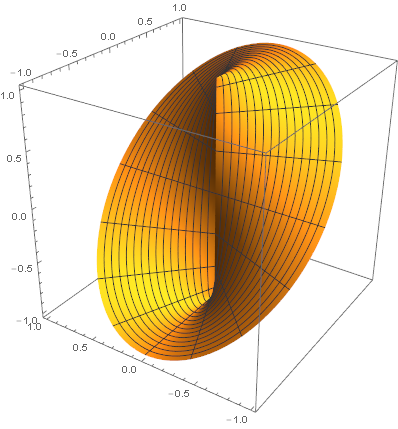
\includegraphics[height=0.3\textheight]{Figures20190609/COSTHETA-1.png} }}
	\subfloat[]{\label{costheta-2}
{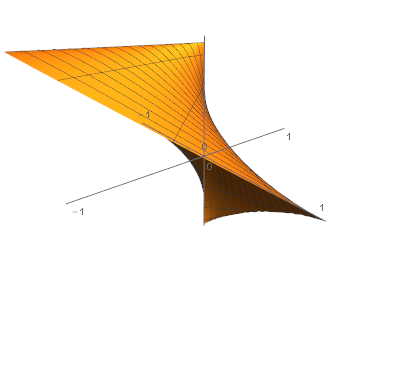
\includegraphics[height=0.3\textheight]{Figures20190609/COSTHETA-2.png} }}
\end{center}
\caption{函数$f(r\cos\theta,r\sin\theta)=\cos\theta,(r,\theta)\in\Set{(r,\theta)}{0<r\leqslant1,0\leqslant\theta\leqslant2\pi}$的图形}
\label{costheta}
\end{figure}
\end{enumerate}
\subsection{习题11.1解答}
\begin{enumerate}
\item设$\bm u(t),\bm v(t)$是可导的向量值函数,$\lambda(t)$为可导数值函数,求证:\\
(1)$\frac{\mathrm d}{\mathrm dt}(\lambda(t)\bm u(t))=\frac{\mathrm d\lambda(t)}{\mathrm dt}\bm u(t)+\lambda(t)\frac{\mathrm d}{\mathrm dt}\bm u(t)$;\\
(2)$\frac{\mathrm d}{\mathrm dt}(\bm u(t)\bm\cdot\bm v(t))=(\frac{\mathrm d}{\mathrm dt}\bm u(t))\bm\cdot\bm v(t)+\bm u(t)\bm\cdot(\frac{\mathrm d}{\mathrm dt}\bm v(t))$.

证明:(1)设$\bm u(t)=(u_1(t),u_2(t),u_3(t))$,则$\lambda(t)\bm u(t)=(\lambda(t)u_1(t),\lambda(t)u_2(t),\lambda(t)u_3(t))$,
\[\begin{split}
\frac{\mathrm d}{\mathrm dt}(\lambda(t)\bm u(t))&=({\mathrm dt}[\lambda(t)u_1(t)]',[\lambda(t)u_2(t)]',[\lambda(t)u_3(t)]')\\
&=(\lambda'(t)u_1(t)+\lambda(t)u'_1(t),\lambda'(t)u_2(t)+\lambda(t)u'_2(t),\lambda'(t)u_3(t)+\lambda(t)u'_3(t))\\
&=(\lambda'(t)u_1(t),\lambda'(t)u_2(t),\lambda'(t)u_3(t))+(\lambda(t)u'_1(t),\lambda(t)u'_2(t),\lambda(t)u'_3(t))\\
&=\lambda'(t)(u_1(t),u_2(t),u_3(t))+\lambda(t)(u'_1(t),u'_2(t),u'_3(t))\\
&=\frac{\mathrm d\lambda(t)}{\mathrm dt}\bm u(t)+\lambda(t)\frac{\mathrm d}{\mathrm dt}\bm u(t).
\end{split}\]
(2)设$\bm u(t)=(u_1(t),u_2(t),u_3(t)),\bm v(t)=(v_1(t),v_2(t),v_3(t))$,

则$\bm u(t)\bm\cdot\bm v(t)=u_1(t)v_1(t)+u_2(t)v_2(t)+u_3(t)v_3(t)$,
\[\begin{split}
\frac{\mathrm d}{\mathrm dt}(\bm u(t)\bm\cdot\bm v(t))&=\frac{\mathrm d}{\mathrm dt}[u_1(t)v_1(t)+u_2(t)v_2(t)+u_3(t)v_3(t)]\\
&=u'_1(t)v_1(t)+u_1(t)v'_1(t)+u'_2(t)v_2(t)+u_2(t)v'_2(t)+u'_3(t)v_3(t)+u_3(t)v'_3(t)\\
&=u'_1(t)v_1(t)+u'_2(t)v_2(t)+u'_3(t)v_3(t)+u_1(t)v'_1(t)+u_2(t)v'_2(t)+u_3(t)v'_3(t)\\
&=(\frac{\mathrm d}{\mathrm dt}\bm u(t))\bm\cdot\bm v(t)+\bm u(t)\bm\cdot(\frac{\mathrm d}{\mathrm dt}\bm v(t)).
\end{split}\]
\item求下列曲线在指定点的单位切向量:\\
(1)$\bm r(t)=(\mathrm e^{2t},\mathrm e^{-2t},t\mathrm e^{2t}),t=0$;\\
(2)$\bm r(t)=t\bm i+2\sin t\bm j+3\cos t\bm k,t=\frac\pi6$.

解:(1)单位切向量$\bm t=\frac{\bm r'(t)}{|\bm r'(t)|}=\frac{(2\mathrm e^{2t},-2\mathrm e^{-2t},(1+2t)\mathrm e^{2t})}{\|(2\mathrm e^{2t},-2\mathrm e^{-2t},(1+2t)\mathrm e^{2t})\|}\Big|_{t=0}=\frac{(2,-2,1)}{\sqrt{4+4+1}}=(\frac23,-\frac23,\frac13)$.

(2)单位切向量$\bm t=\frac{\bm r'(t)}{|\bm r'(t)|}=\frac{\bm i+2\cos t\bm j-3\sin t\bm k}{\|\bm i+2\cos t\bm j-3\sin t\bm k\|}\Big|_{t=\frac\pi6}=\frac{\bm i+\sqrt3\bm j-\frac32\bm k}{\sqrt{1+3+\frac94}}=\frac25\bm i+\frac{2\sqrt3}5\bm j-\frac35\bm k$.

\item求下列曲线在指定点的切线方程:\\
(1)$\bm r(t)=(1+2t,1+t-t^2,1-t+t^2-t^3),M(1,1,1)$;\\
(2)$\bm r(t)=\sin(\pi t)\bm i+\sqrt t\bm j+\cos(\pi t)\bm k,M(0,1,-1)$.

解:(1)在$M(1,1,1)$点处$t=0$,切向量$\bm t=\bm r'(0)=(2,1-2t,-1+2t-3t^2)_{t=0}=(2,1,-1)$,则切线方程为
\[\frac{x-1}2=y-1=-(z-1).\]
(2)在$M(0,1,-1)$点处$t=1$,切向量$\bm t=\bm r'(1)=\pi\cos(\pi t)\bm i+\frac1{2\sqrt t}\bm j-\pi\sin(\pi t)\bm k\big|_{t=1}=-\pi\bm i+\frac12\bm j$,则切线方程为$\begin{cases}
\frac x{-\pi}=2(y-1),\\
z=-1,
\end{cases}$即$\begin{cases}
x+2\pi y=2\pi,\\
z=-1.
\end{cases}$

\item求下列向量值函数的积分:\\
(1)$\int_0^{\frac\pi4}[\cos(2t)\bm i+\sin(2t)\bm j+t\sin t\bm k]\mathrm dt$;\\
(2)$\int_1^4(\sqrt t\bm i+t\mathrm e^{-t}\bm j+\frac1{t^2}\bm k)\mathrm dt$.

解:(1)$\int_0^{\frac\pi4}[\cos(2t)\bm i+\sin(2t)\bm j+t\sin t\bm k]\mathrm dt=\int_0^{\frac\pi4}\cos(2t)\mathrm dt\bm i+\int_0^{\frac\pi4}\sin(2t)\mathrm dt\bm j+\int_0^{\frac\pi4}t\sin t\mathrm dt\bm k$,

$\because\int_0^{\frac\pi4}\cos(2t)\mathrm dt=\frac12\sin(2t)\big|_0^{\frac\pi4}=\frac12,\ \int_0^{\frac\pi4}\sin(2t)\mathrm dt=-\frac12\cos(2t)\big|_0^{\frac\pi4}=\frac12,\\
\int_0^{\frac\pi4}t\sin t\mathrm dt=-\int_0^{\frac\pi4}t\mathrm d\cos t=-t\cos t\big|_0^{\frac\pi4}+\int_0^{\frac\pi4}\cos t\mathrm dt=-\frac{\sqrt2\pi}{8}+\sin t\big|_0^{\frac\pi4}=-\frac{\sqrt2\pi}{8}+\frac{\sqrt2}2$,

$\therefore\int_0^{\frac\pi4}[\cos(2t)\bm i+\sin(2t)\bm j+t\sin t\bm k]\mathrm dt=\frac12\bm i+\frac12\bm j+(-\frac{\sqrt2\pi}{8}+\frac{\sqrt2}2)\bm k$.

(2)$\int_1^4(\sqrt t\bm i+t\mathrm e^{-t}\bm j+\frac1{t^2}\bm k)\mathrm dt=\int_1^4\sqrt t\mathrm dt\bm i+\int_1^4t\mathrm e^{-t}\mathrm dt\bm j+\int_1^4\frac1{t^2}\mathrm dt\bm k$,

$\because\int_1^4\sqrt t\mathrm dt=\frac1{1+\frac12}t^{\frac12+1}\big|_1^4=\frac{14}3,\int_1^4t\mathrm e^{-t}\mathrm dt=-\int_1^4t\mathrm d\mathrm e^{-t}=-t\mathrm e^{-t}\big|_1^4+\int_1^4\mathrm e^{-t}\mathrm dt\\
=-4\mathrm e^{-4}+\mathrm e^{-1}-\mathrm e^{-t}\big|_1^4=-4\mathrm e^{-4}+\mathrm e^{-1}-\mathrm e^{-4}+\mathrm e^{-1}=-5\mathrm e^{-4}+2\mathrm e^{-1},\\
\int_1^4\frac1{t^2}\mathrm dt=\frac1{-2+1}t^{-2+1}\big|_1^4=-\frac14+1=\frac34$,

$\therefore\int_1^4(\sqrt t\bm i+t\mathrm e^{-t}\bm j+\frac1{t^2}\bm k)\mathrm dt=\frac{14}3\bm i+(-5\mathrm e^{-4}+2\mathrm e^{-1})\bm j+\frac34\bm k$.

\item已知$\bm r'(t),\bm r(0)$,求$\bm r(t)$:\\
(1)$\bm r'(t)=(t^2,4t^3,-t^2),\bm r(0)=(0,1,0)$;\\
(2)$\bm r'(t)=\sin t\bm i-\cos t\bm j+2t\bm k,\bm r(0)=\bm i+\bm j+2\bm k$.

解:(1)方法1:
\[\begin{split}
\bm r(t)&=\int_0^t\bm r'(t)\mathrm dt+\bm C=(\int_0^tt^2\mathrm dt+C_1,\int_0^t4t^3\mathrm dt+C_2,\int_0^t(-t^2)\mathrm dt+C_3)\\
&=(\frac13t^3+C_1,t^4+C_2,-\frac13t^3+C_3),
\end{split}\]
$\therefore\bm r(0)=(C_1,C_2,C_3)=(0,1,0)$,

$\therefore\bm r(t)=(\frac13t^3,t^4+1,-\frac13t^3)$.

方法2:$\because\int t^2\mathrm dt=\frac13t^3+C,\ \int4t^3\mathrm dt=t^4+C,\ \int(-t^2)\mathrm dt=-\frac13t^3+C$,

$\therefore r(t)=\int\bm r'(t)\mathrm dt=(\frac13t^3+C_1,t^4+C_2,-\frac13t^3+C_3)$,

$\because\bm r(0)=(0,1,0)$,

$\therefore C_1=0,\ C_2=1,\ C_3=0$,

$\therefore\bm r(t)=(\frac13t^3,t^4+1,-\frac13t^3)$.

(2)方法1:\[\begin{split}
\bm r(t)=&\int_0^t\bm r'(t)\mathrm dt+\bm C=(\int_0^t\sin t\mathrm dt+C_1)\bm i+(-\int_0^t\cos t\mathrm dt+C_2)\bm j+(\int_0^t2t\mathrm dt+C_3)\bm k\\
=&(-\cos t+C_1)\bm i+(-\sin t+C_2)\bm j+(t^2+C_3)\bm k,
\end{split}\]
$\because\bm r(0)=(-1+C_1)\bm i+C_2\bm j+C_3\bm k=\bm i+\bm j+2\bm k$,

$\therefore C_1=2,C_2=1,C_3=2$,

$\therefore\bm r(t)=(-\cos t+2)\bm i+(-\sin t+1)\bm j+(t^3+2)\bm k$.

方法2:$\because\int\sin t\mathrm dt=-\cos t+C,\ \int(-\cos t)\mathrm dt=-\sin t+C,\ \int2t\mathrm dt=t^2+C$,

$\therefore\bm r(t)=\int\bm r'(t)\mathrm dt=(-\cos t+C_1)\bm i+(-\sin t+C_2)\bm j+(t^2+C_3)\bm k$,

$\because\bm r(0)=\bm i+\bm j+2\bm k$,

$\therefore C_1=2,\ C_2=1,\ C_3=2$,

$\therefore\bm r(t)=(-\cos t+2)\bm i+(-\sin t+1)\bm j+(t^3+2)\bm k$.

\item证明下列等式:\\
(1)$\frac{\mathrm d}{\mathrm dt}(\bm r(t)\times\bm r'(t))=\bm r(t)\times\bm r''(t)$;\\
(2)$\frac{\mathrm d}{\mathrm dt}\|\bm r(t)\|=\frac{\bm r(t)\bm\cdot\bm r'(t)}{\|\bm r(t)\|}(\bm r(t)\neq\bm0)$;\\
(3)$\frac{\mathrm d}{\mathrm dt}[\bm r(t)\bm\cdot(\bm r'(t)\times\bm r''(t))]=\bm r(t)\bm\cdot[\bm r'(t)\times\bm r'''(t)]$.

证明:(1)$\frac{\mathrm d}{\mathrm dt}(\bm r(t)\times\bm r'(t))=\bm r'(t)\times\bm r'(t)+\bm r(t)\times\bm r''(t)=\bm r(t)\times\bm r''(t)$.

(2)$\frac{\mathrm d}{\mathrm dt}\|\bm r(t)\|=\frac{\mathrm d}{\mathrm dt}\sqrt{\bm r(t)\bm\cdot\bm r(t)}=\frac1{2\sqrt{\bm r(t)\bm\cdot\bm r(t)}}\frac{\mathrm d}{\mathrm dt}[\bm r(t)\bm\cdot\bm r(t)]\\
=\frac1{2\sqrt{\bm r(t)\bm\cdot\bm r(t)}}[\bm r'(t)\bm\cdot\bm r(t)+\bm r(t)\bm\cdot\bm r'(t)]=\frac{2\bm r(t)\bm\cdot\bm r'(t)}{2\sqrt{\bm r(t)\bm\cdot\bm r(t)}}=\frac{\bm r(t)\bm\cdot\bm r'(t)}{\|\bm r(t)\|}(\bm r(t)\neq\bm0)$.

(3)$\frac{\mathrm d}{\mathrm dt}[\bm r(t)\bm\cdot(\bm r'(t)\times\bm r''(t))]=\bm r'(t)\bm\cdot(\bm r'(t)\times\bm r''(t))+\bm r(t)\bm\cdot\frac{\mathrm d}{\mathrm dt}(\bm r'(t)\times\bm r''(t))\\
=\bm r(t)\bm\cdot\frac{\mathrm d}{\mathrm dt}(\bm r'(t)\times\bm r''(t))=\bm r(t)\bm\cdot(\bm r''(t)\times\bm r''(t)+\bm r'(t)\times\bm r'''(t))=\bm r(t)\bm\cdot[\bm r'(t)\times\bm r'''(t)]$.

\item求等速圆周运动$\bm r=R\cos(\omega t)\bm i+R\sin(\omega t)\bm j$在$t$时刻的速度与加速度.

解:$t$时刻的速度$\bm v(t)=\bm r'(t)=-R\omega\sin(\omega t)\bm i+R\omega\cos(\omega t)\bm j$,

$t$时刻的加速度$\bm a(t)=\bm v'(t)=-R\omega^2\cos(\omega t)\bm i-R\omega^2\sin(\omega t)\bm j$.

\item已知螺旋线的向量方程为$\bm r=a\cos\theta\bm i+a\sin\theta\bm j+b\theta\bm k(a>0,b>0)$,求在$\theta_0$处的切线方程.

解:在$\theta_0$处的切向量$\bm r'(\theta_0)=-a\sin\theta_0\bm i+a\cos\theta_0\bm j+b\bm k$,切线方程
\[\frac{x-a\cos\theta_0}{-a\sin\theta_0}=\frac{y-a\sin\theta_0}{a\cos\theta_0}=\frac{z-b\theta_0}b.\]

\item设$\bm r=-a\sin\theta\bm i+a\cos\theta\bm j+b\theta\bm k$,求$\frac12\int_0^{2\pi}(\bm r\times\bm r')\mathrm d\theta$.

解:$\bm r'(\theta)=-a\cos\theta\bm i-a\sin\theta\bm j+b\bm k$,

$\bm r(\theta)\times\bm r'(\theta)=\begin{vmatrix}
\bm i&\bm j&\bm k\\
-a\sin\theta&a\cos\theta&b\theta\\
-a\cos\theta&-a\sin\theta&b
\end{vmatrix}=\begin{vmatrix}
a\cos\theta&b\theta\\
-a\sin\theta&b
\end{vmatrix}\bm i+\begin{vmatrix}
b\theta&-a\sin\theta\\
b&-a\cos\theta
\end{vmatrix}\bm j+\begin{vmatrix}
-a\sin\theta&a\cos\theta\\
-a\cos\theta&-a\sin\theta
\end{vmatrix}\bm k\\
=(ab\cos\theta+ab\theta\sin\theta)\bm i-(-ab\sin\theta+ab\theta\cos\theta)\bm j+a^2\bm k$,

$\because\int_0^{2\pi}(ab\cos\theta+ab\theta\sin\theta)\mathrm d\theta=ab\sin\theta\big|_0^{2\pi}-\int_0^{2\pi}ab\theta\mathrm d\cos\theta\\
=-ab\theta\cos\theta\big|_0^{2\pi}+\int_0^{2\pi}ab\cos\theta\mathrm d\theta=-2\pi ab+ab\sin\theta\big|_0^{2\pi}=-2\pi ab,\\
\int_0^{2\pi}-(-ab\sin\theta+ab\theta\cos\theta)\mathrm d\theta=\int_0^{2\pi}(ab\sin\theta-ab\theta\cos\theta)\mathrm d\theta=-ab\cos\theta\big|_0^{2\pi}-ab\int_0^{2\pi}\theta\mathrm d\sin\theta\\
=-ab\theta\sin\theta\big|_0^{2\pi}+ab\int_0^{2\pi}\sin\theta\mathrm d\theta=-ab\cos\theta\big|_0^{2\pi}=0,\\
\int_0^{2\pi}a^2\mathrm d\theta=2\pi a^2$,

$\therefore\frac12\int_0^{2\pi}(\bm r\times\bm r')\mathrm d\theta=-\pi ab\bm i+\pi a^2\bm k$.
\end{enumerate}
\end{document}